\problemname{Jan Ersa}
This is how a poem by Gustaf Fröding begins:\\
{\em
Jan Ersa ägde Nackabyn,\\
Per Persa ägde Backabyn \\
i By i Västra Ed. \\
Jan Ersa, \\
Per Persa, \\
de höllo aldrig fred.
}

When Jan Ersa and Per Persa, in their old age, moved into the city, they made sure to end up as far
away from each other as possible. Write a program that reads information about the streets in the city and then
determines between which two houses the shortest path is the longest, and then outputs the houses and the length of this path.
All streets are bidirectional.

\begin{figure}[ht!]
  \centering
  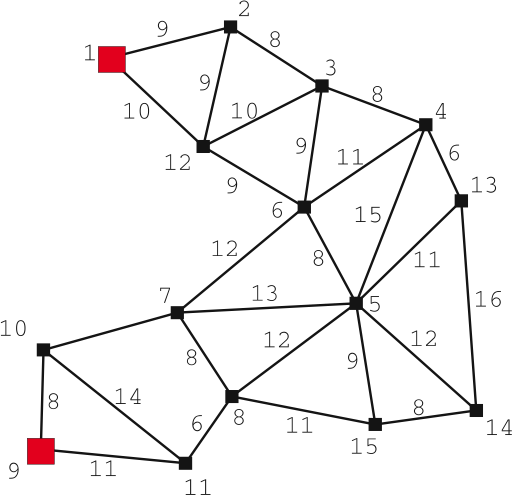
\includegraphics[width=0.4\textwidth]{janersa.png}
  \caption{The map shows all houses and streets of the city in the example. We also see the red houses where Jan Ersa and Per Persa now live. These two houses (numbers 1 and 9) are the houses in the city that are farthest away from each other (4900 meters).}
\end{figure}


\section*{Input}
The first line contains the integer $N$ ($2 \le N \le 700$), the number of houses in the city. The houses are numbered from $1$ to $N$.

The second line contains the integer $V$ ($1 \le V \le 2000$), the number of streets.

The following $V$ lines each contain the integers $a$, $b$, $l$ ($1 \leq a,b \leq N$, $a \neq b$, $1 \leq l \leq 100$),
describing that there is a street between houses $a$ and $b$ with length $l$ (given in hundreds of meters).
There is at most one street between each pair of houses.
It is guaranteed that it is possible to get from any house to any other house.

\section*{Output}
Print three integers on one line: the numbers of the two houses farthest away from each other, and the distance between them in meters.
If there are several pairs of houses at this distance, you may output any of them.

\section*{Scoring}
Your solution will be tested on a set of test groups.
To earn points for a group, you must pass all test cases in that group.

\noindent
\begin{tabular}{| l | l | p{12cm} |}
  \hline
  \textbf{Group} & \textbf{Points} & \textbf{Constraints} \\ \hline
  $1$    & $30$       & $N \leq 25, V \leq 75$ \\ \hline
  $2$    & $70$       & No additional constraints. \\ \hline
\end{tabular}
